\documentclass[12pt,a4paper,twoside]{article}
\usepackage{fancyhdr,graphicx,latexsym}

\setlength{\parindent}{0cm}
\setlength{\parskip}{2ex plus1ex minus 0.5ex}

\addtolength{\evensidemargin}{-2.5cm}
\addtolength{\oddsidemargin}{-0.5cm}
\addtolength{\textwidth}{3cm}

\addtolength{\headheight}{0.2cm}
\addtolength{\topmargin}{-1cm}
\addtolength{\textheight}{2.5cm}

\renewcommand{\_}{\texttt{\symbol{95}}}
\addtolength{\fboxsep}{0.1cm}
\newcommand{\param}[1]{\textit{\textrm{\textmd{#1}}}}
\newcommand{\codebar}{\rule{\textwidth}{0.3mm}}
% \newcommand{\spc}{\hspace{0.5mm}$\sqcup$\hspace{0.6mm}}
\newcommand{\spc}{\hspace{0.5mm}$\Box$\hspace{0.5mm}}
\newcommand{\todo}[1]{\textbf{TODO: #1}}

\newlength{\codelen}
\newcommand{\code}[1]
{\begin{center}\fbox{\parbox{16cm}{\texttt{#1}}}\end{center}}

\fancyhead{}
\fancyhead[RO,LE]{\thepage}
\fancyhead[LO,RE]{SBUS Prebuilt Components}
\fancyfoot{}
\pagestyle{empty}

\newenvironment{bulletlist}
{
	\begin{itemize}
	\setlength{\itemsep}{0ex}
	\setlength{\parsep}{0ex}
}
{
	\end{itemize}
}

\newenvironment{alphalist}
{
	\begin{enumerate}
	\setlength{\itemsep}{0ex}
	\setlength{\parsep}{0ex}
	\renewcommand{\labelenumi}{(\alph{enumi})}
}
{
	\end{enumerate}
}

\newenvironment{numericlist}
{
	\begin{enumerate}
	\setlength{\itemsep}{0ex}
	\setlength{\parsep}{0ex}
}
{
	\end{enumerate}
}

\begin{document}

% \sfseries
\centerline{\textbf{\LARGE SBUS Prebuilt Components}}
\begin{center} \large
David Ingram\\
TIME-EACM Project\\
University of Cambridge Computer Lab\\
4th July 2007\\
\end{center}

{ \parskip 1mm plus 1pt \tableofcontents }
\pagestyle{fancy}

\section{Introduction}

This document describes some standard reusable pre-built components.
The resource discovery component is significant enough to be covered
in another document.

\textbf{Note:} Of the components listed here, \textit{only} the first
(the event broker component) is currently implemented and ships
as part of the SBUS distribution.

\section{Broker component}
\label{broker}

This is a general-purpose event broker, supporting topic and content-based
subscriptions. It is trivial to implement, needing one sink endpoint which
accepts any message, and one source which outputs everything
received. The wrapper's built-in subscription matching takes care of
the rest; content and topic based subscriptions are possible.

This component is polymorphic, because its endpoints handle
messages of any type (specfied by the \verb^"*"^ schema).
Actual schemas are needed for all messages received, in order to parse
the binary encoding into an \verb^snode^ which can then be matched
by the subscription. These are retrieved via the built-in
\verb^lookup_schema()^ endpoint.

% \begin{figure}[htbp]
\begin{figure}[ht]
\centering
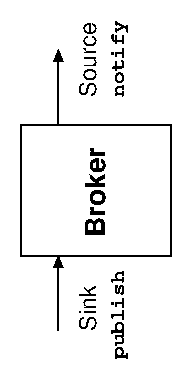
\includegraphics[scale=1.0,angle=-90]{diagrams/broker.eps}
% \caption{Communication types}
% \label{broker}
\end{figure}

\section{Selector component}

Filter a generic stream based on a sub-tree (say location)
without disturbing the rest of the tree. Requires the
sub-tree matching extension.

\section{Bridge component}

Connect to a given endpoint, and echo messages out as a new stream
with identical types (retransmit with same hash codes).
This is mainly useful as a test of the ability to handle messages
of any type without possessing the schema needed to decode them.

Note: the broker component already does this, so do we still need
a bridge?

\section{Standard I/O adapter component}

\todo{Specify this in detail}

XML (+hash value?) or line-based strings (wrapped or unwrapped)
type unknown/ASCII

\begin{bulletlist}
\item Possible interface:
   \texttt{stdout} emits new stream, \texttt{stdin} collects stream
   data subscribed to, \texttt{stderr} specifies subscriptions
	(incoming streams will be interleaved with this interface, so must
	be in XML if there is more than one of them)

\item Stream sources should be designed to output in XML to \texttt{stdout}
   (note: some added complexity due to the need to find the
   message document end-tags before passing parts of the stream to the XML
   parser to build a DOM)
\end{bulletlist}

\section{Object store component}

This is an XML database. It is suitable for storing configuration
information, mapping data and ontologies etc.
The storage space is structured as a single large XML document,
addressed by paths from the root, e.g. \verb^foo/bar^.
Path components may consist of the \verb^*^ wildcard.

Service endpoints:
\begin{bulletlist}
\item \verb^update^ -- add or alter data
\item \verb^read^ -- returns a subtree
\item \verb^list^ -- returns the top-level members within the path specified
\item \verb^delete^
\item \verb^listen^ -- returns events containing changes to the subtree of
	the database you are interested in
\end{bulletlist}

\section{Stream persistence component}

This component can be instantiated to connect to a named stream and
record its data persistently (a common requirement), offering a
timespan (replay) API.

You must specify the stream to record (component and endpoint) and a directory
to use for storage when starting the persistence component.

Output is provided by a server endpoint with the API below.
Storage is append-only (hence direct file read access is also permissable
for local processes).

\begin{verbatim}
replay(^timeslice)

   @timeslice
   {
      [ clk from ]
      [ clk to ]
   }
\end{verbatim}

Either \verb^from^ or \verb^to^ can be omitted. An end-of-stream
OOB packet is sent at the end (unless there is no stopping point).

Note: a generic replay storage implementation cannot necessarily
extract any stream-specific timestamp information from each message.
The timestamps it associates with an event are therefore not the
same as message-internal timestamps, instead they are the time
as recorded by the storage component when each message arrives
from the stream.

To consider: History conversion plugins for on-the-fly conversion to
support a multi-facet API? Problem: some things cannot be converted due
to missing information and non-equivalence.

\section{Demux component}

This is a demultiplexer, which listens on a single open port and connects
through to other ports internally.
It is useful when firewall admin will only open one port, and for use with
SSH port forwarding.

\begin{figure}[htbp]
\centering
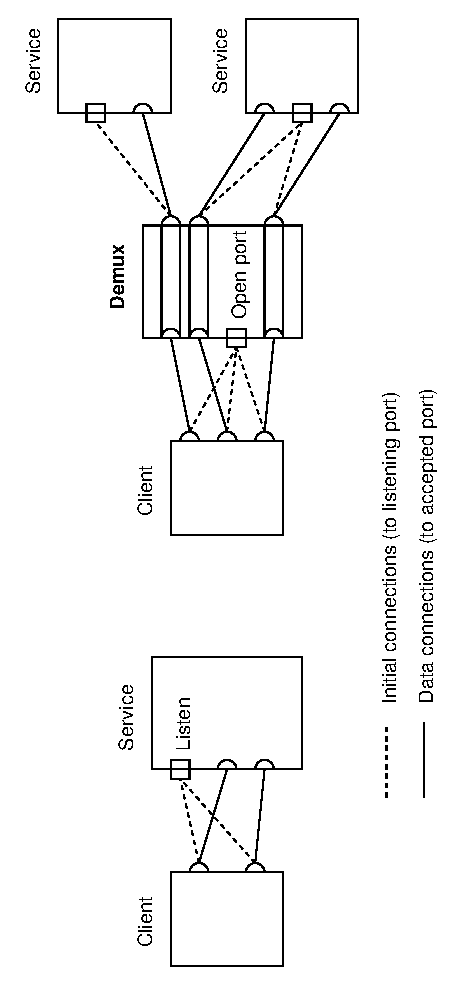
\includegraphics[scale=1.0,angle=-90]{diagrams/demux.eps}
% \caption{Communication types}
\label{demux}
\end{figure}

\textbf{Interaction with the RDC}

A RDC will normally be \textit{inside} the firewall.
Hence the RDC must be accessed through the demux as well.

Clients need to know the demux address so that they can contact
the RDC and all components behind it.

\end{document}
